\documentclass{standalone}
\usepackage{tikz}
\usetikzlibrary{patterns, positioning}


\begin{document}
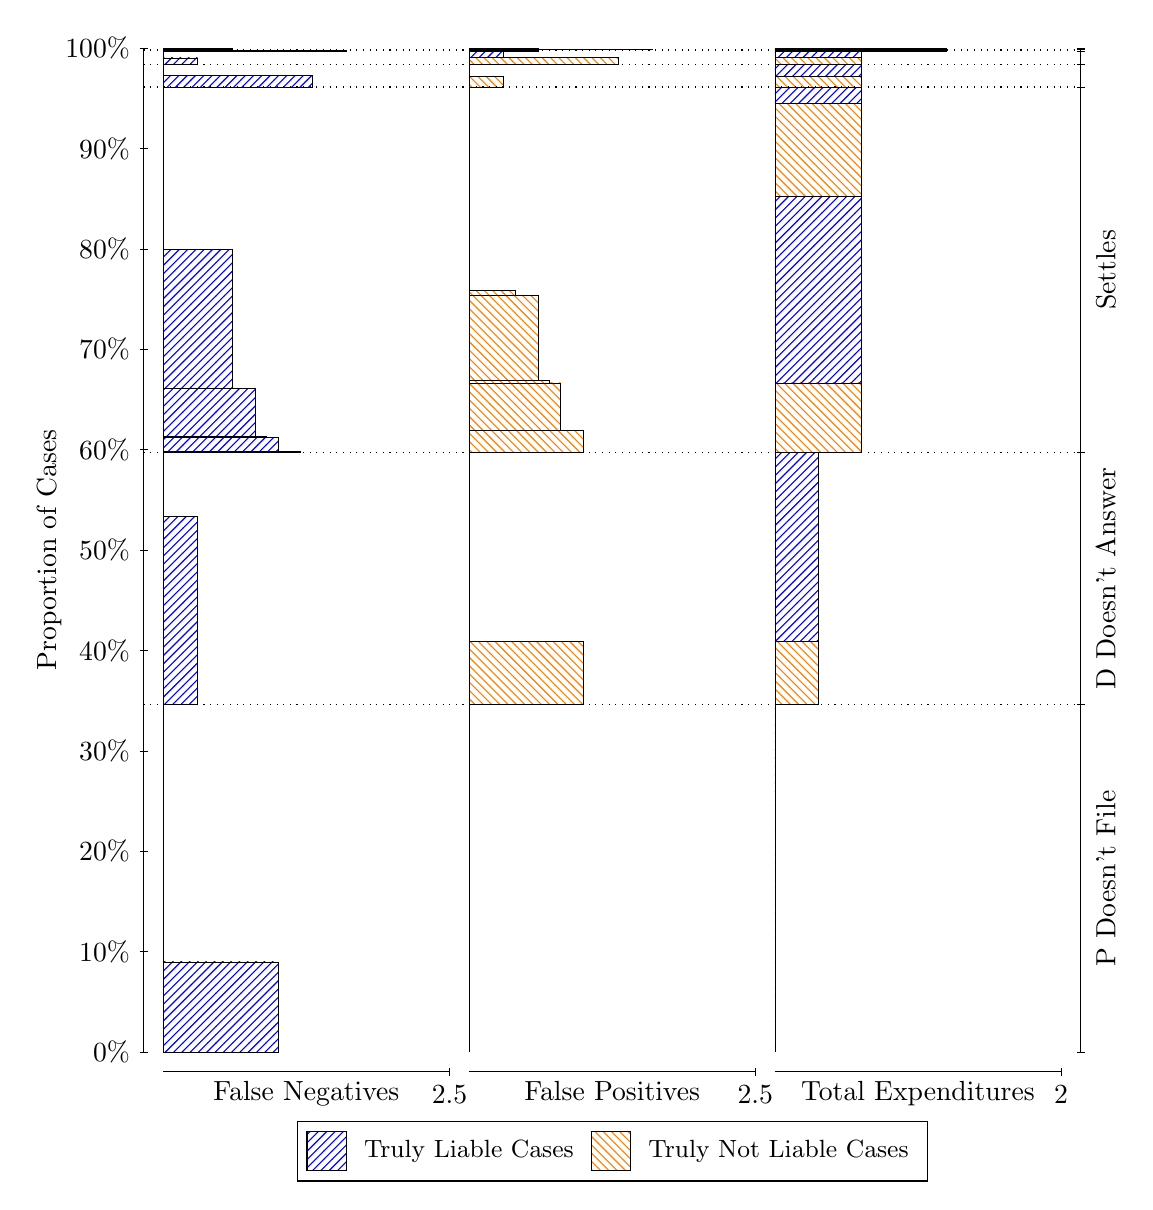
\begin{tikzpicture}
\draw[black, very thin] (1.5,1.75) -- (1.5,14.5);
\node[rotate=90, text=black, anchor=center] at (0.3, 8.125) {Proportion of Cases};
\draw[black, very thin] (1.45,1.75) -- (1.55,1.75);
\node[text=black, anchor=east] at (1.45, 1.75) {0\%};
\draw[black, very thin] (1.45,3.025) -- (1.55,3.025);
\node[text=black, anchor=east] at (1.45, 3.025) {10\%};
\draw[black, very thin] (1.45,4.3) -- (1.55,4.3);
\node[text=black, anchor=east] at (1.45, 4.3) {20\%};
\draw[black, very thin] (1.45,5.575) -- (1.55,5.575);
\node[text=black, anchor=east] at (1.45, 5.575) {30\%};
\draw[black, very thin] (1.45,6.85) -- (1.55,6.85);
\node[text=black, anchor=east] at (1.45, 6.85) {40\%};
\draw[black, very thin] (1.45,8.125) -- (1.55,8.125);
\node[text=black, anchor=east] at (1.45, 8.125) {50\%};
\draw[black, very thin] (1.45,9.4) -- (1.55,9.4);
\node[text=black, anchor=east] at (1.45, 9.4) {60\%};
\draw[black, very thin] (1.45,10.675) -- (1.55,10.675);
\node[text=black, anchor=east] at (1.45, 10.675) {70\%};
\draw[black, very thin] (1.45,11.95) -- (1.55,11.95);
\node[text=black, anchor=east] at (1.45, 11.95) {80\%};
\draw[black, very thin] (1.45,13.225) -- (1.55,13.225);
\node[text=black, anchor=east] at (1.45, 13.225) {90\%};
\draw[black, very thin] (1.45,14.5) -- (1.55,14.5);
\node[text=black, anchor=east] at (1.45, 14.5) {100\%};

\draw[black, very thin] (13.4,1.75) -- (13.4,14.5);
\draw[black, very thin] (13.35,1.75) -- (13.45,1.75);
\node[anchor=west] at (13.35, 1.75) {};
\draw[black, very thin] (13.35,6.16) -- (13.45,6.16);
\node[anchor=west] at (13.35, 6.16) {};
\draw[black, very thin] (13.35,9.3608) -- (13.45,9.3608);
\node[anchor=west] at (13.35, 9.3608) {};
\draw[black, very thin] (13.35,14.005) -- (13.45,14.005);
\node[anchor=west] at (13.35, 14.005) {};
\draw[black, very thin] (13.35,14.288) -- (13.45,14.288);
\node[anchor=west] at (13.35, 14.288) {};
\draw[black, very thin] (13.35,14.465) -- (13.45,14.465);
\node[anchor=west] at (13.35, 14.465) {};
\draw[black, very thin] (13.35,14.481) -- (13.45,14.481);
\node[anchor=west] at (13.35, 14.481) {};
\draw[black, very thin] (13.35,14.5) -- (13.45,14.5);
\node[anchor=west] at (13.35, 14.5) {};

\draw[black, very thin, pattern color=blue, pattern=north east lines] (1.75,1.75) rectangle (3.2033,2.895);
\draw[black, very thin, pattern color=orange, pattern=north west lines] (1.75,2.895) rectangle (1.75,6.16);
\draw[black, very thin, pattern color=blue, pattern=north east lines] (1.75,6.16) rectangle (2.186,8.5554);
\draw[black, very thin, pattern color=orange, pattern=north west lines] (1.75,8.5554) rectangle (1.75,9.3608);
\draw[black, very thin, pattern color=blue, pattern=north east lines] (1.75,9.3608) rectangle (3.494,9.377);
\draw[black, very thin, pattern color=blue, pattern=north east lines] (1.75,9.377) rectangle (3.2033,9.5571);
\draw[black, very thin, pattern color=blue, pattern=north east lines] (1.75,9.5571) rectangle (3.058,9.572);
\draw[black, very thin, pattern color=blue, pattern=north east lines] (1.75,9.572) rectangle (2.9127,10.177);
\draw[black, very thin, pattern color=blue, pattern=north east lines] (1.75,10.177) rectangle (2.622,11.943);
\draw[black, very thin, pattern color=orange, pattern=north west lines] (1.75,11.943) rectangle (1.75,14.005);
\draw[black, very thin, pattern color=blue, pattern=north east lines] (1.75,14.005) rectangle (3.6393,14.151);
\draw[black, very thin, pattern color=orange, pattern=north west lines] (1.75,14.151) rectangle (1.75,14.288);
\draw[black, very thin, pattern color=blue, pattern=north east lines] (1.75,14.288) rectangle (2.186,14.375);
\draw[black, very thin, pattern color=orange, pattern=north west lines] (1.75,14.375) rectangle (1.75,14.465);
\draw[black, very thin, pattern color=blue, pattern=north east lines] (1.75,14.465) rectangle (4.0753,14.47);
\draw[black, very thin, pattern color=orange, pattern=north west lines] (1.75,14.47) rectangle (1.75,14.481);
\draw[black, very thin, pattern color=blue, pattern=north east lines] (1.75,14.481) rectangle (2.622,14.495);
\draw[black, very thin, pattern color=orange, pattern=north west lines] (1.75,14.495) rectangle (1.75,14.5);
\draw[black, very thin, pattern color=orange, pattern=north west lines] (5.6333,1.75) rectangle (5.6333,5.015);
\draw[black, very thin, pattern color=blue, pattern=north east lines] (5.6333,5.015) rectangle (5.6333,6.16);
\draw[black, very thin, pattern color=orange, pattern=north west lines] (5.6333,6.16) rectangle (7.0867,6.9654);
\draw[black, very thin, pattern color=blue, pattern=north east lines] (5.6333,6.9654) rectangle (5.6333,9.3608);
\draw[black, very thin, pattern color=orange, pattern=north west lines] (5.6333,9.3608) rectangle (7.0867,9.6408);
\draw[black, very thin, pattern color=orange, pattern=north west lines] (5.6333,9.6408) rectangle (6.796,10.248);
\draw[black, very thin, pattern color=orange, pattern=north west lines] (5.6333,10.248) rectangle (6.6507,10.277);
\draw[black, very thin, pattern color=orange, pattern=north west lines] (5.6333,10.277) rectangle (6.5053,11.363);
\draw[black, very thin, pattern color=orange, pattern=north west lines] (5.6333,11.363) rectangle (6.2147,11.423);
\draw[black, very thin, pattern color=blue, pattern=north east lines] (5.6333,11.423) rectangle (5.6333,14.005);
\draw[black, very thin, pattern color=orange, pattern=north west lines] (5.6333,14.005) rectangle (6.0693,14.142);
\draw[black, very thin, pattern color=blue, pattern=north east lines] (5.6333,14.142) rectangle (5.6333,14.288);
\draw[black, very thin, pattern color=orange, pattern=north west lines] (5.6333,14.288) rectangle (7.5227,14.378);
\draw[black, very thin, pattern color=blue, pattern=north east lines] (5.6333,14.378) rectangle (6.0693,14.465);
\draw[black, very thin, pattern color=orange, pattern=north west lines] (5.6333,14.465) rectangle (6.5053,14.475);
\draw[black, very thin, pattern color=blue, pattern=north east lines] (5.6333,14.475) rectangle (5.6333,14.481);
\draw[black, very thin, pattern color=orange, pattern=north west lines] (5.6333,14.481) rectangle (7.9587,14.486);
\draw[black, very thin, pattern color=blue, pattern=north east lines] (5.6333,14.486) rectangle (6.5053,14.5);
\draw[black, very thin, pattern color=orange, pattern=north west lines] (9.5167,1.75) rectangle (9.5167,5.015);
\draw[black, very thin, pattern color=blue, pattern=north east lines] (9.5167,5.015) rectangle (9.5167,6.16);
\draw[black, very thin, pattern color=orange, pattern=north west lines] (9.5167,6.16) rectangle (10.062,6.9654);
\draw[black, very thin, pattern color=blue, pattern=north east lines] (9.5167,6.9654) rectangle (10.062,9.3608);
\draw[black, very thin, pattern color=orange, pattern=north west lines] (9.5167,9.3608) rectangle (10.607,10.248);
\draw[black, very thin, pattern color=blue, pattern=north east lines] (9.5167,10.248) rectangle (10.607,12.618);
\draw[black, very thin, pattern color=orange, pattern=north west lines] (9.5167,12.618) rectangle (10.607,13.793);
\draw[black, very thin, pattern color=blue, pattern=north east lines] (9.5167,13.793) rectangle (10.607,14.005);
\draw[black, very thin, pattern color=orange, pattern=north west lines] (9.5167,14.005) rectangle (10.607,14.142);
\draw[black, very thin, pattern color=blue, pattern=north east lines] (9.5167,14.142) rectangle (10.607,14.288);
\draw[black, very thin, pattern color=orange, pattern=north west lines] (9.5167,14.288) rectangle (10.607,14.378);
\draw[black, very thin, pattern color=blue, pattern=north east lines] (9.5167,14.378) rectangle (10.607,14.465);
\draw[black, very thin, pattern color=orange, pattern=north west lines] (9.5167,14.465) rectangle (11.697,14.475);
\draw[black, very thin, pattern color=blue, pattern=north east lines] (9.5167,14.475) rectangle (11.697,14.481);
\draw[black, very thin, pattern color=orange, pattern=north west lines] (9.5167,14.481) rectangle (11.697,14.486);
\draw[black, very thin, pattern color=blue, pattern=north east lines] (9.5167,14.486) rectangle (11.697,14.5);
\draw[black, dotted] (1.5,6.16) -- (13.4,6.16);
\draw[black, dotted] (1.5,9.3608) -- (13.4,9.3608);
\draw[black, dotted] (1.5,14.005) -- (13.4,14.005);
\draw[black, dotted] (1.5,14.288) -- (13.4,14.288);
\draw[black, dotted] (1.5,14.465) -- (13.4,14.465);
\draw[black, dotted] (1.5,14.481) -- (13.4,14.481);
\draw[black, very thin] (1.75,1.5) -- (5.3833,1.5);
\node[text=black, anchor=north] at (3.5667, 1.5) {False Negatives};
\draw[black, very thin] (5.3833,1.45) -- (5.3833,1.55);
\node[text=black, anchor=north] at (5.3833, 1.45) {2.5};

\draw[black, very thin] (5.6333,1.5) -- (9.2667,1.5);
\node[text=black, anchor=north] at (7.45, 1.5) {False Positives};
\draw[black, very thin] (9.2667,1.45) -- (9.2667,1.55);
\node[text=black, anchor=north] at (9.2667, 1.45) {2.5};

\draw[black, very thin] (9.5167,1.5) -- (13.15,1.5);
\node[text=black, anchor=north] at (11.333, 1.5) {Total Expenditures};
\draw[black, very thin] (13.15,1.45) -- (13.15,1.55);
\node[text=black, anchor=north] at (13.15, 1.45) {2};

\node[text=black, centered, rotate=90] at (13.72, 3.955) {P Doesn't File};
\node[text=black, centered, rotate=90] at (13.72, 7.7604) {D Doesn't Answer};
\node[text=black, centered, rotate=90] at (13.72, 11.683) {Settles};





\draw (7.449999999999999,1.5) node[draw=none] (baseCoordinate) {};
\begin{scope}[align=center]
        \matrix[scale=0.5, draw=black, below=0.5cm of baseCoordinate, nodes={draw}, column sep=0.1cm]{
            \node[rectangle, draw, minimum width=0.5cm, minimum height=0.5cm, pattern color=blue, pattern=north east lines] {}; &
            \node[draw=none, font=\small, text=black] (B) {Truly Liable Cases}; &
            \node[rectangle, draw, minimum width=0.5cm, minimum height=0.5cm, pattern color=orange, pattern=north west lines] {}; &
            \node[draw=none, font=\small, text=black] (B) {Truly Not Liable Cases}; \\
            };
\end{scope}

\end{tikzpicture}
\end{document}